% Unofficial Georgia Tech Psychology Poster Template
% based on
% https://github.com/k4rtik/uchicago-poster
% a fork of https://github.com/anishathalye/gemini

\documentclass[final]{beamer}

% ====================
% Packages
% ====================

\usepackage[T1]{fontenc}
\usepackage{lmodern}
\usepackage[size=custom,width=121cm,height=91cm,scale=1.0]{beamerposter}
\usetheme{gemini}
\usecolortheme{gatech}
\usepackage{graphicx}
\usepackage{atbegshi}
\AtBeginDocument{\AtBeginShipoutNext{\AtBeginShipoutDiscard}}
\usepackage{booktabs}
\usepackage{doi}
\usepackage{natbib}
\usepackage[patch=none]{microtype}
\usepackage{tikz}
\usepackage{pgfplots}
\usepackage{subfig}
\usepackage{qrcode}
\usepackage{hyperref}
\pgfplotsset{compat=1.18}
\usepackage{anyfontsize}

\pdfstringdefDisableCommands{%
\def\translate#1{#1}%
}

% ====================
% Lengths
% ====================

% If you have N columns, choose \sepwidth and \colwidth such that
% (N+1)*\sepwidth + N*\colwidth = \paperwidth
\newlength{\sepwidth}
\newlength{\colwidth}
\setlength{\sepwidth}{0.025\paperwidth}
\setlength{\colwidth}{0.3\paperwidth}

\newcommand{\separatorcolumn}{\begin{column}{\sepwidth}\end{column}}

% ====================
% Title
% ====================

\title{Approaching Sudoku Symmetry Groups Using Group Theory (MATH 466)}

\author{\LARGE\textbf{Jimmy Sitompul}}


% ====================
% Footer (optional)
% ====================

\footercontent{
  \Large \textbf{Department of Mathematics} \hfill \Large \textbf{Colorado State University}
  \hfill
  \href{mailto:jimmy.sitompul@colostate.edu}{jimmy.sitompul@colostate.edu}}
% (can be left out to remove footer)

% ====================
% Logo (optional)
% change logos in header by replacing the png files
% ====================


% ====================
% Body
% ====================

\begin{document}
\addtobeamertemplate{headline}{}
{
    \begin{tikzpicture}[remember picture, overlay]
      \node [anchor=north west, inner sep=3cm] at ([xshift=0.0cm,yshift=2.5cm]current page.north west)
      {
\includegraphics[height=6.0cm]{pic/Math-NS-CSU-1-H357.png}};
      \node [anchor=north east, inner sep=3cm] at ([xshift=0.0cm,yshift=2.5cm]current page.north east)
      {
\includegraphics[height=6.0cm]{pic/Math-NS-CSU-1-H357.png}};
    \end{tikzpicture}
}

\begin{frame}[t]
\begin{columns}[t]
\separatorcolumn

\begin{column}{\colwidth}

  \begin{alertblock}{\Large What Is Sudoku?}
      \large Sudoku is a $9 \times 9$ grid Latin square puzzle.
      \vspace{\baselineskip}
      \begin{figure}
        \centering
        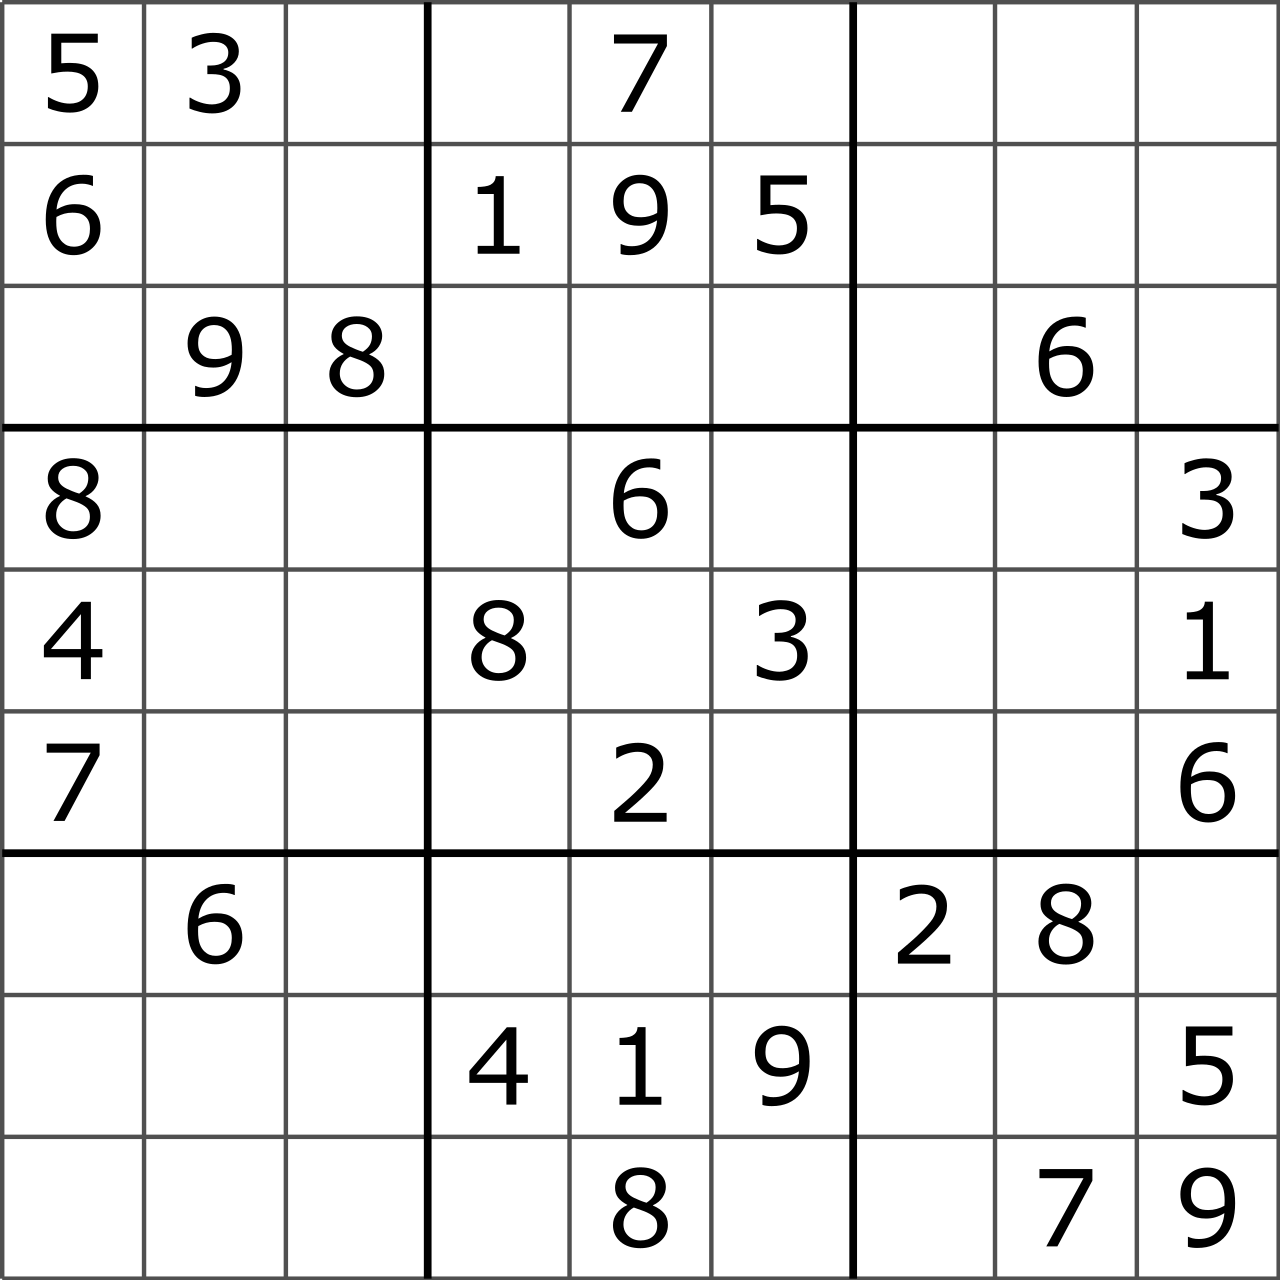
\includegraphics[scale=0.25]{pic/sudokutable.png}
        \caption{A Sudoku puzzle}
        \label{fig:my_label}
    \end{figure}
    \textbf{Objective:}\\
    \large Fill the $9\times9$ grid with numbers $1$ to $9$ in each cell so that \underline{no number} appears twice in:
    \begin{enumerate}
        \item each of the nine rows.
        \item each of the nine columns.
        \item each of the nine $3 \times 3$ subgrids (or \textbf{blocks}).
    \end{enumerate}
  \end{alertblock}
  


  \begin{block}{\Large Connection to Group Theory}
   \large We will use the concepts of:
   \begin{enumerate}
       \item The \textbf{dihedral group} $D_4$ which contains $8$ symmetries of a square diamond, generated by the \textbf{rotation} $r$ and the \textbf{reflection} $s$.
       \item The composition of \textbf{permutations}.
       \item The \textbf{group action}, where the motions of rotation $r$ and of reflection $s$ act on the set f vertices of the square.
   \end{enumerate}
  \end{block}

  

\begin{alertblock}{\Large Sudoku "Puzzle" vs Sudoku "Board"}
\large
\begin{itemize}
    \item A \textbf{Sudoku board} is a $9\times9$ grid that is already filled with the numbers $1$ to $9$ according to the rules of the game.
    \item A \textbf{Sudoku puzzle} is any subset of a Sudoku board (the unsolved one).
\end{itemize}
    
  \end{alertblock}

\begin{block}{\Large Bands and Stacks in Sudoku}
\large
\begin{itemize}
    \item \textbf{Bands} are the three $3$-row strips, whereas \textbf{stacks} are the three $3$-column strips.
    \item We \textbf{cannot} interchange two rows that are not in the same band and similarly interchange two columns that are not in the same stack.
    \item However, we \textbf{can} interchange two rows that are in the same band and two columns that are in the same stack, as well as interchanging any two entire bands and any two entire stacks.
\end{itemize} 
\begin{figure}
        \centering
        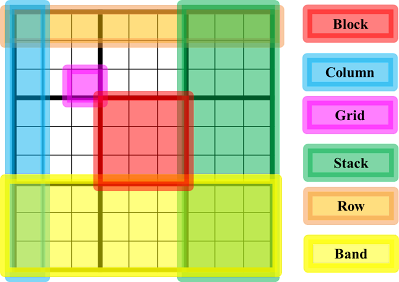
\includegraphics[scale=1.2]{pic/SudokuNotation.png}
        \caption{Glossary of Sudoku}
        \label{fig:my_label}
    \end{figure}
    
  \end{block}

  
  

\end{column}

\separatorcolumn

\begin{column}{\colwidth}

\begin{alertblock}{\Large "Essentially The Same" Sudokus}
   \large Two Sudoku boards A and B are \textbf{essentially the same} if there exists a Sudoku symmetry $g \in G$ such that $g$ applied to B yields C.
  \end{alertblock}



\begin{block}{\Large Are These Sudoku Puzzles "Essentially the Same"?}
    \begin{figure}
       \centering
       \subfloat[\centering Sudoku A]{{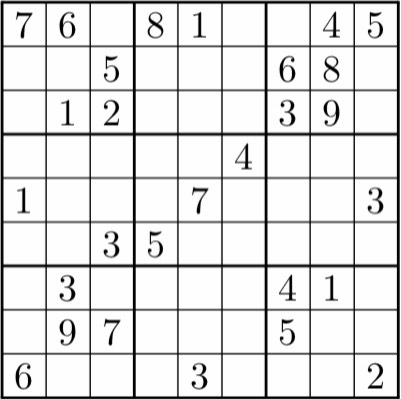
\includegraphics[scale=0.8]{pic/IMG_0941.jpg} }}
       \quad \quad \quad 
       \subfloat[\centering Sudoku B]{{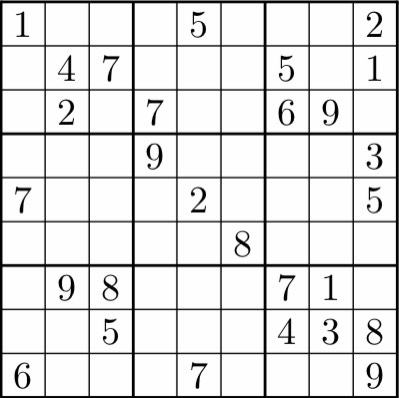
\includegraphics[scale=0.8]{pic/IMG_0942.jpg }}}
   \end{figure}
  \end{block}

\begin{alertblock}{\Large Algorithm Similarity}

    \large \heading{Sudoku A}\\ 
   Suppose that we want to put $3$ in the first row of Sudoku A, the algorithm that successfully puts $3$ in the first row is:
   \begin{enumerate}
       \item The $3^{rd}, 6^{th},$ and the $7^{th}$ cell are empty.
       \item The third column already has a $3$ and the top right block also contains $3$.
       \item Therefore, $3$ should be placed in the $6^{th}$ cell of the first row.
   \end{enumerate}
   \heading{Sudoku B}\\
   Now, suppose that we want to put $7$ in the last column of Sudoku B, the algorithm that successfully puts $7$ in the last column is:
   \begin{enumerate}
       \item The $3^{rd}, 6^{th},$ and the $7^{th}$ cell are empty.
       \item The third row already has a $7$ and the bottom right block also contains $7$.
       \item Therefore, $7$ should be placed in the $6^{th}$ cell of the last column.
   \end{enumerate}
  \end{alertblock}
\begin{block}{\Large Déjà vu?}
  \large \large Do you think we have a similar algorithm? We do have! This shows that Sudoku A is \textbf{"essentially the same"} as Sudoku B. \\
  \vspace{\baselineskip}
  To sum up, Sudoku A and Sudoku B are the same puzzle, but here Sudoku A is \textbf{\underline{rotated $90^{\circ}$ clockwise}} and the numbers are then \textbf{\underline{relabelled by the permutation cycle}} $(159483726)$.
  \end{block} 

  \begin{alertblock}{\Large Sudoku Symmetry Group Actions}
    \large Here, we can consider the similar group of actions on Sudoku boards that include the actions above. The elements of actions are $\{ r,s,B_{12},B_{13},R_{12},R_{13} \}$, where
    \begin{itemize}
        \item $B_{mn}$ is defined by the swap of band $m$ with band $n$.
        \item $R_{mn}$ is defined by the swap of row $m$ with row $n$.
    \end{itemize}
    \end{alertblock}

    \begin{alertblock}{\Large Definition: Sudoku Symmetry Group}
        The generators of all Sudoku symmetries are $\{B_{12},R_{12}, r \}$, together with relabelling the numbers in the cells which has $9!$ possible ways to do, represented by the group $S_9$. Therefore, The \textbf{Sudoku symmetry group} is $G = \langle B_{12},R_{12}, r \rangle \times S_9$
    \end{alertblock}
    

\end{column}

\separatorcolumn

\begin{column}{\colwidth}

    \begin{block}{\Large Examples}
        \large The group actions on Sudoku boards can be written as a combination of the generators $\{B_{12},R_{12}, r \}$:
        \begin{align*}
            B_{13} &= r^2 \circ B_{12} \circ r^2 \\
            R_{13} &= B_{12} \circ r^2 \circ R_{12} \circ r^2 \circ B_{12}\\
            s &= r \circ B_{12} \circ r^2 \circ B_{12} \circ r^2 \circ R_{12} \circ B_{12} \circ r^2 \circ R_{12} \circ B_{12} \circ r^2 \circ R_{12} \circ B_{12} \circ r^2 \circ R_{12} \\  & \ \ \ \ \circ B_{12} \circ r^2 \circ R_{12} \circ B_{12} \circ r^2 \circ R_{12} \circ B_{12} \circ R_{12} \circ r^2 \circ R_{12} \circ B_{12} \circ R_{12}
        \end{align*}
        
    \end{block}

    \begin{alertblock}{\Large How Big is Sudoku Symmetry Group?}
        The size of Sudoku symmetry group is $2 \cdot (3!)^8 \cdot 9! =1,218,998,108,160$, where $2 \cdot (3!)^8 $ is the size of group actions $\{ r,s,B_{12},B_{13},R_{12},R_{13} \}$ and $9!$ is the size of the group $S_9$.
    \end{alertblock}


    \begin{block}{\Large Sudoku Symmetry and Solving Symmetry}
    \begin{figure}
        \centering
        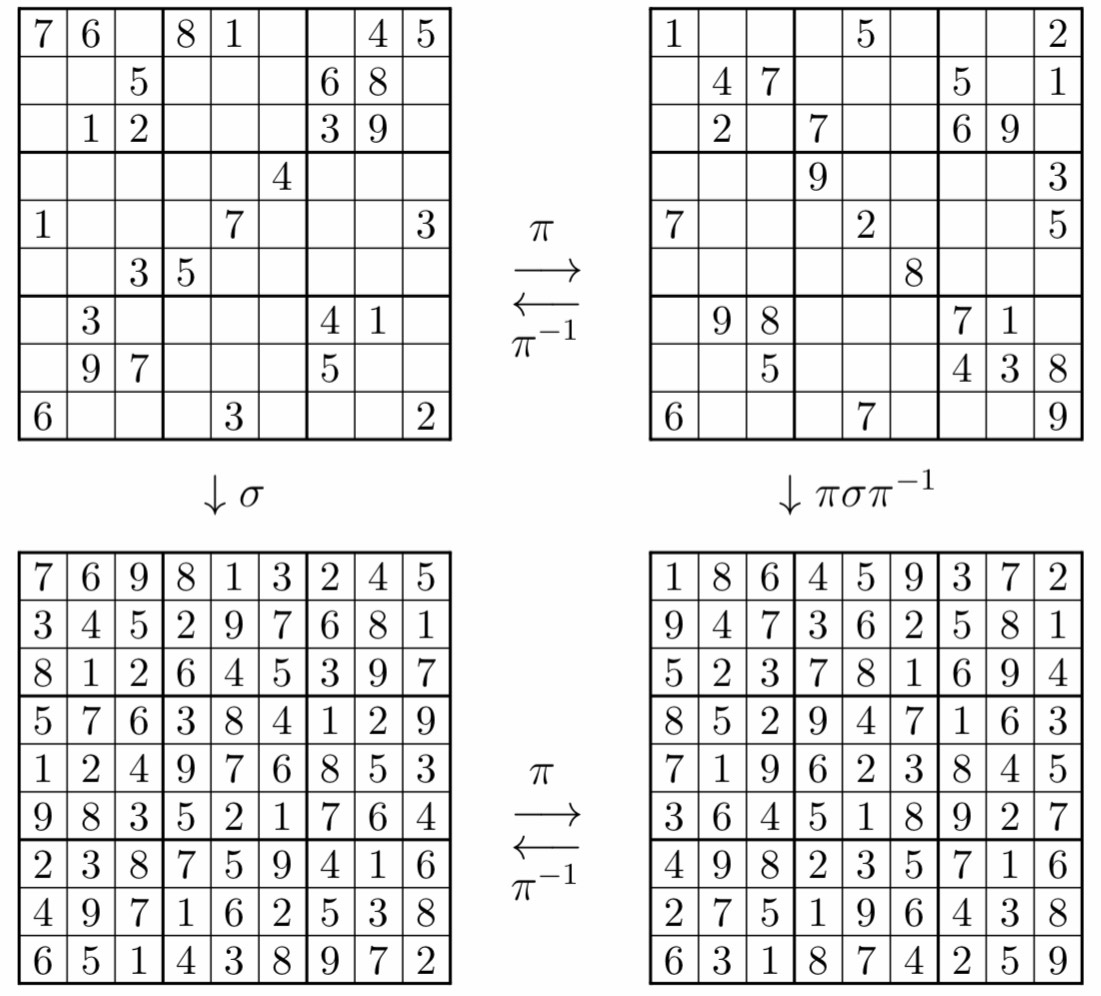
\includegraphics[scale=0.65]{pic/IMG_0943.jpg}
        \caption{The Sudoku symmetry $\pi$ and the solving symmetry $\sigma$}
        \label{fig:my_label}
    \end{figure}
    \large Here, we define $\pi=r \circ (159483726)$ and we have $\pi(A)=B$. The solving symmetry $\sigma$ completes Sudoku A to become Sudoku C and $\pi^{-1}\sigma\pi$, which the same solving symmetry as $\sigma$, completes Sudoku B to become Sudoku D.
  \end{block}


  \begin{alertblock}{\Large Acknowledgement}

    Jimmy Sitompul, the author of MATH466 project, acknowledges that this project includes general ideas and intuitions about the topic, as well as previous research paper regarding the chosen topic. Jimmy Sitompul would also like to thank the MATH466 Instructor, Dr. Rachel Pries, for assigning this task to all the students. 
    
  \end{alertblock}

  \begin{alertblock}{\Large References}

    \begin{thebibliography}{10}
        \bibitem{arnold1} Arnold, E., Chapman, H., and Rupert, M., "How Do You Solve Sudoku? A Group-theoretic Approach to Human Solving Strategies," pp. 1-16, \href{http://www.jimrolf.com/explorationsInComplexVariables/explorationsComplexVariables6.7.11.pdf}{http://www.jimrolf.com/explorationsInComplexVariables/explorationsComplexVariables6.7.11.pdf}
        \bibitem{gromley} Gromley, Kevin, "Generalizing Sudoku Strategies," pp. 1-13, 2014, \href{https://www.sudokuwiki.org/sudoku/Generalizing_Sudoku_Strategies.pdf}{https://www.sudokuwiki.org/sudoku/Generalizing$_$Sudoku$_$Strategies.pdf}
        \bibitem{sudoku} Wikipedia, "Sudoku," 2022, \href{https://en.wikipedia.org/wiki/Sudoku}{https://en.wikipedia.org/wiki/Sudoku}
    \end{thebibliography}

  \end{alertblock}

  \large \textbf{Scan this barcode to play Sudoku:} \quad \quad
  \qrcode[height=2in]{https://sudoku.com/}



\end{column}

\separatorcolumn
\end{columns}
\end{frame} 

\end{document}